%%%%%%%%%%%%%%%%%%%%%%%%%%%%%%%%%%%%

\section{1.6. Estatística Descritiva, resumindo a informação contida}

%%%%%% d%%dade %os%%%%% no banco%%%%%%%%%%%%%%%%%%%%%%

\subsection{Gráficos de dispersão para dados pareados}

%%%%%%%%%%%%%%%%%%%%%%%%%%%%%%%%%%%%

\begin{frame}
\frametitle{Gráficos de dispersão}
\justifying
\hl{Gráficos de dispersão} são úteis para visualizar a relação entre duas variáveis numéricas.

\begin{columns}[c]

\column{0.6 \textwidth}
\justifying
\dq{A expectativa de vida e a fertilidade total parecem ser \hl {associadas} ou \hl {independentes}?}
\justifying
\soln{\onslide<2->{Eles parecem estar linearmente e negativamente associadas: à medida que a fertilidade aumenta, a expectativa de vida diminui.}}
\justifying
\dq{O associação foi a mesma ao longo dos anos, ou mudou?}
\justifying
\soln{\onslide<3->{A associação entre elas mudou ao longo dos anos.}}

\column{0.4 \textwidth}

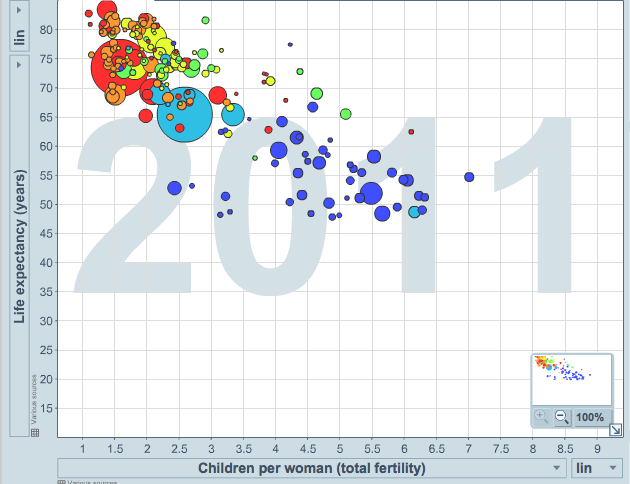
\includegraphics[width=\textwidth]{1-6_numerical_data/figures/life_exp_child.png}

\end{columns}

\ct{\webURL{http://www.gapminder.org/world}}

\end{frame}

%%%%%%%%%%%%%%%%%%%%%%%%%%%%%%%%%%%%

\subsection{Parcelas de pontos e a média}

%%%%%%%%%%%%%%%%%%%%%%%%%%%%%%%%%%%%

\begin{frame}
\frametitle{Gráfico}
\justifying
Útil para visualizar uma variável numérica. Cores mais escuras representam áreas onde há mais observações.

\begin{center}
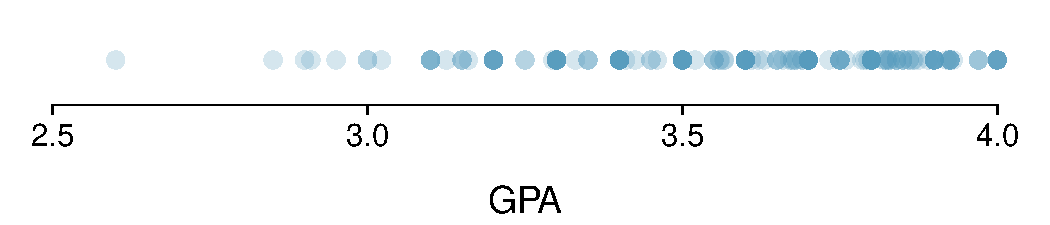
\includegraphics[width=\textwidth]{1-6_numerical_data/gpa_dot_plot.pdf}
\end{center}
\justifying
\dq{Como você descreveria a distribuição de GPAs nesse conjunto de dados? É possível indicar um ponto central ou a forma da distribuição desses dados?}

\end{frame}

%%%%%%%%%%%%%%%%%%%%%%%%%%%%%%%%%%%%


\begin{frame}
\frametitle{Gráfico}

\begin{center}
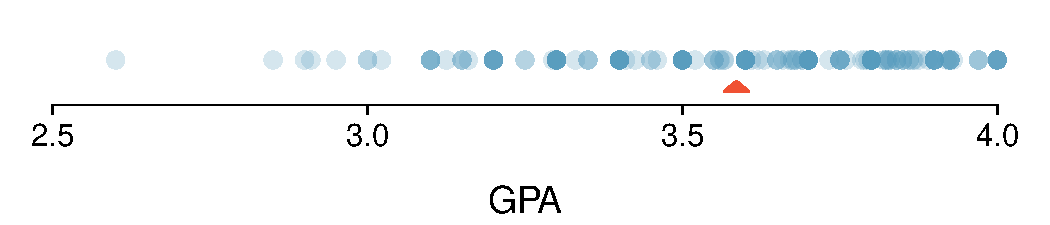
\includegraphics[width=\textwidth]{1-6_numerical_data/gpa_dot_plot_mean.pdf}
\end{center}

\begin{itemize}
\justifying
\item A \hl {média} (marcada com um triângulo no gráfico acima), é uma maneira de medir o centro de uma \hl {distribuição}.
\justifying
\item A média do GPA é de 3,59.

\end{itemize} 

\end{frame}

%%%%%%%%%%%%%%%%%%%%%%%%%%%%%%%%%%%%

\begin{frame}
\frametitle{Média}

\begin{itemize}
\justifying
\item A \hl {média da amostra}, denotada como \mathhl {\bar {x}}, pode ser calculada como

$$
\bar{x} = \frac{x_1 + x_2 + \cdots + x_n}{n},
$$

em que $x_1, x_2, \cdots, x_n$ representa as \hl{n} variáveis observadas.

\justifying
\item A \hl{média populacional} também é calculada da mesma maneira, mas é denotada como $\mathhl{\mu}$. Muitas vezes, não é possível calcular $\mu$, já que não temos informação sobre toda a população (censo).
\justifying
\item A média calculada com os dados da amostra é uma \hl{estatística} e serve como uma \hl{estimativa pontual} da média da população. Sua estimativa pode não ser perfeita, mas se a amostra for representativa da população, \hl{espera-se} que o resultado esteja próximo do verdadeiro valor populacional ($\mu$). 

\end{itemize}

\end{frame}

%%%%%%%%%%%%%%%%%%%%%%%%%%%%%%%%%%%%

\begin{frame}
\frametitle{Gráfico de pontos 2 }
\justifying
Barras mais altas representam áreas onde há mais observações, fica mais fácil visualizar o centro e a forma da distribuição.

\begin{center}
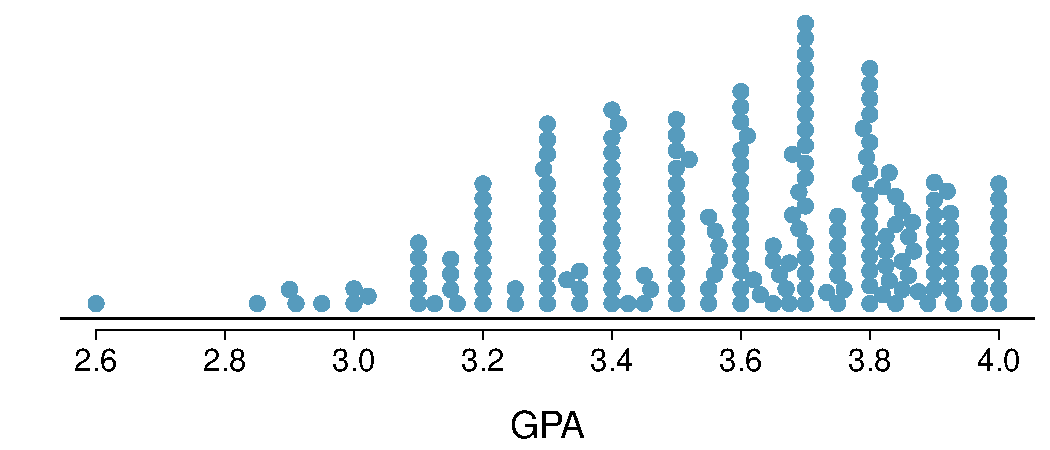
\includegraphics[width=\textwidth]{1-6_numerical_data/gpa_dot_plot_stacked.pdf}
\end{center}

\end{frame}

%%%%%%%%%%%%%%%%%%%%%%%%%%%%%%%%%%%%

\subsection{Histogramas}

%%%%%%%%%%%%%%%%%%%%%%%%%%%%%%%%%%%%

\begin{frame}[fragile]
\frametitle{Histogramas - horas extracurriculares}

\begin{itemize}
\justifying
\item Histogramas fornecem uma visão da \hl{densidade dos dados}. Barras mais altas representam onde os dados são relativamente mais comuns.
\justifying
\item Os histogramas são especialmente convenientes para descrever a \hl{forma} da distribuição dos dados.
\justifying
\item Importante destacar que dependendo da \hl{largura dos intervalos das caixas}, a história que o histograma está contando pode ser alterada drasticamente.

\end{itemize}

\begin{center}
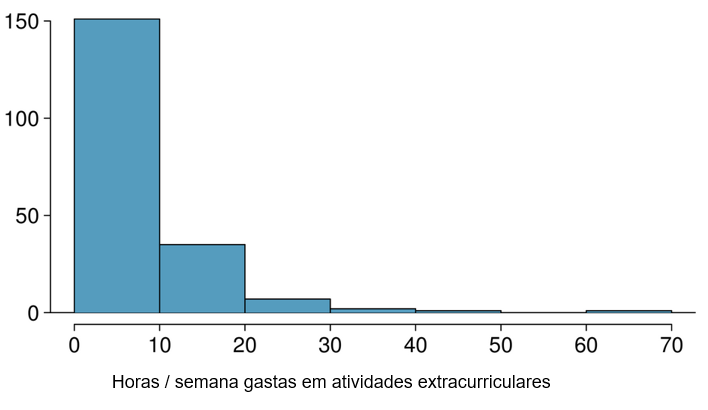
\includegraphics[width=0.60\textwidth]{1-6_numerical_data/extracurr_hrs_hist.png}
\end{center}

\end{frame}

%%%%%%%%%%%%%%%%%%%%%%%%%%%%%%%%%%%%

\begin{frame}
\frametitle{Largura dos intervalos das caixas}
\justifying
\dq{Qual (is) destes histogramas são úteis? Quais revelam muito sobre os dados? Quais escondem muito?}

\begin{center}
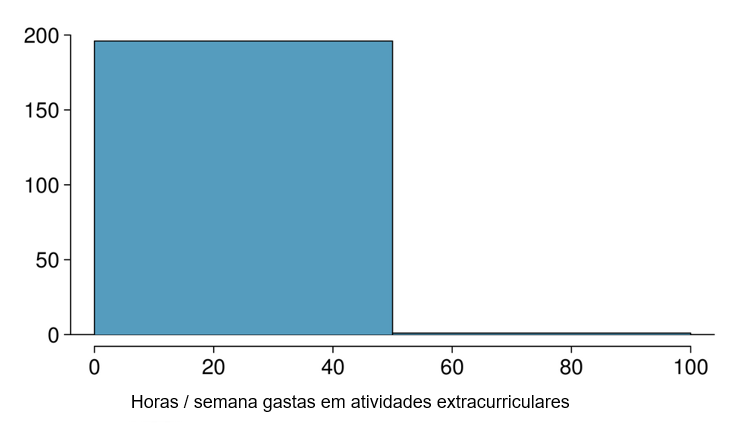
\includegraphics[width=0.45\textwidth]{1-6_numerical_data/extracurr_hrs_hist2.png}
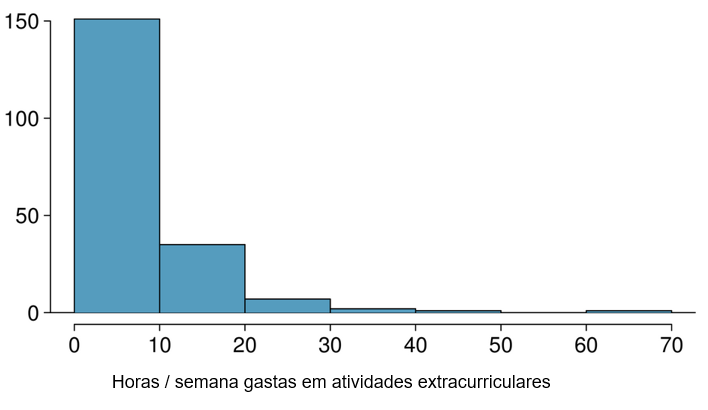
\includegraphics[width=0.45\textwidth]{1-6_numerical_data/extracurr_hrs_hist.png} \\
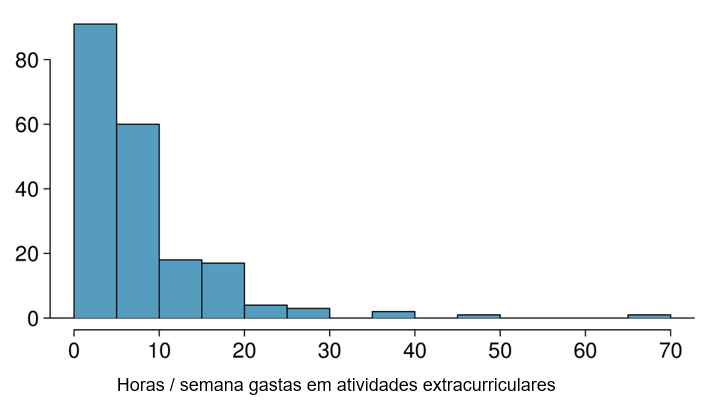
\includegraphics[width=0.45\textwidth]{1-6_numerical_data/extracurr_hrs_hist20.png}
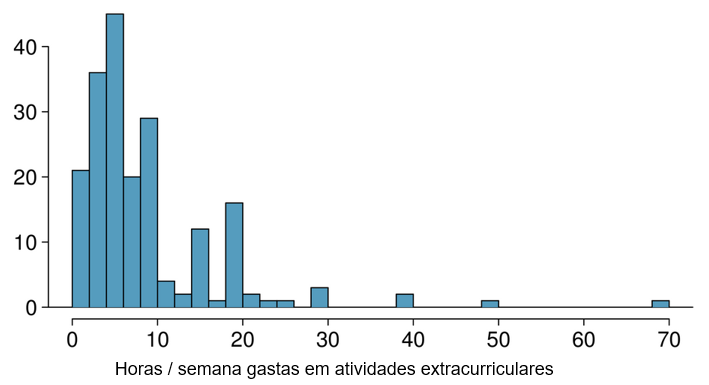
\includegraphics[width=0.45\textwidth]{1-6_numerical_data/extracurr_hrs_hist30.png}
\end{center}

\end{frame}

%%%%%%%%%%%%%%%%%%%%%%%%%%%%%%%%%%%%

\begin{frame}
\frametitle{Distribuição: moda}
\justifying
O histograma pode ter um único pico (\hl{unimodal}), vários picos proeminentes (\hl{bimodal/ multimodal}), ou sem picos aparentes (\hl{uniforme})?

\begin{center}
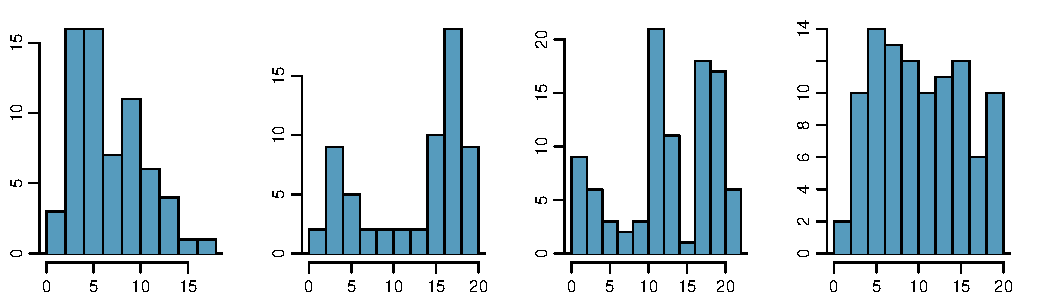
\includegraphics[width=0.75\textwidth]{1-6_numerical_data/singleBiMultiModalUnifPlots.pdf}
\end{center}
\justifying
\Note{Para determinar a moda,  imagine uma curva suave sobre o histograma - imagine que as barras sejam blocos de madeira e você jogue um espaguete mole sobre elas, a forma que o espaguete tomaria pode ser vista como uma curva suave.}

\end{frame}

%%%%%%%%%%%%%%%%%%%%%%%%%%%%%%%%%%%%

\begin{frame}
\frametitle{Distribuição: simetria}
\justifying
O histograma é \hl{assimétrico à direita}, \hl{assimétrico à esquerda}, ou \hl{simétrico}?

\begin{center}
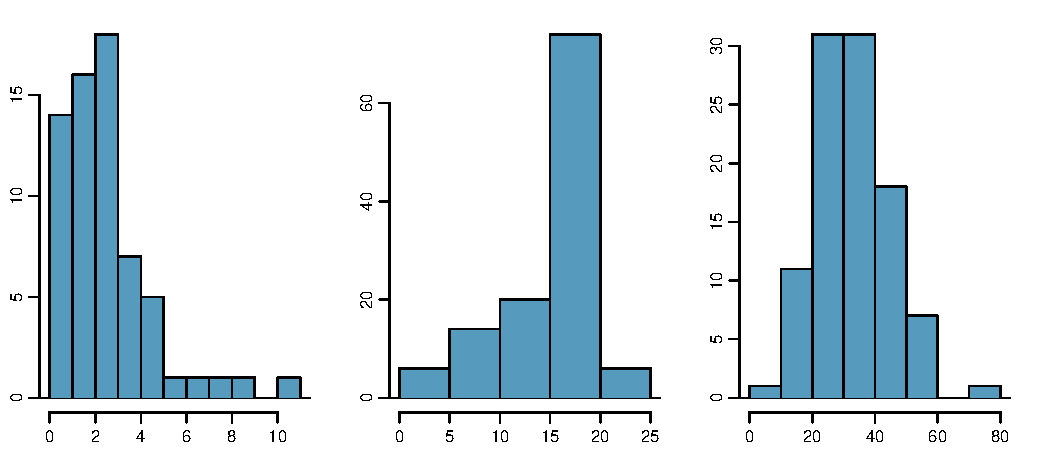
\includegraphics[width=0.8\textwidth]{1-6_numerical_data/skewedSymPlots.pdf}
\end{center}
\justifying
\Note{Observe para qual lado a calda da distribuição está.}

\end{frame}

%%%%%%%%%%%%%%%%%%%%%%%%%%%%%%%%%%%%

\begin{frame}
\frametitle{Forma de distribuição: observações incomuns}
\justifying
Há alguma observação incomum ou potencial \hl{outliers}?

\begin{center}
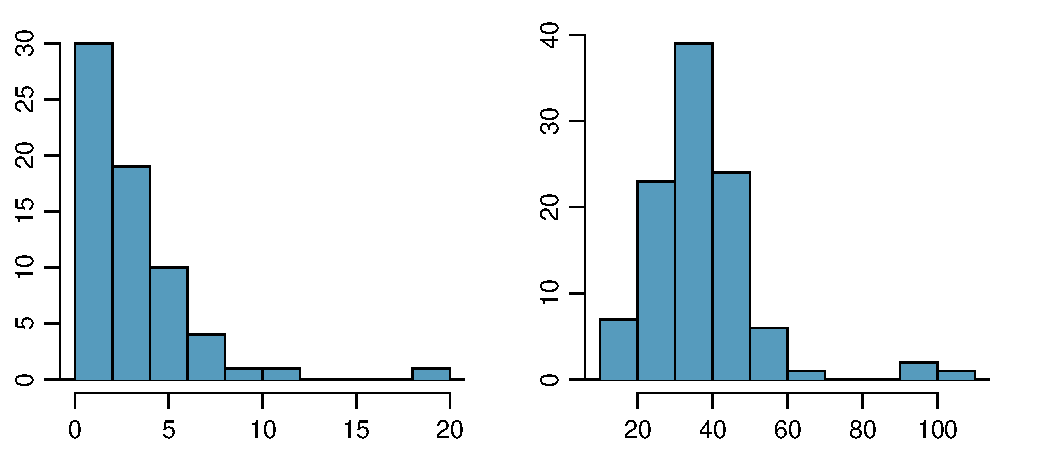
\includegraphics[width=0.8\textwidth]{1-6_numerical_data/outlierPlots.pdf}
\end{center}

\end{frame}

%%%%%%%%%%%%%%%%%%%%%%%%%%%%%%%%%%%%

\begin{frame}
\frametitle{Atividades extracurriculares}
\justifying
\dq{Como você descreveria a forma da distribuição das horas semanais em atividades extracurriculares de estudantes?}

\begin{center}
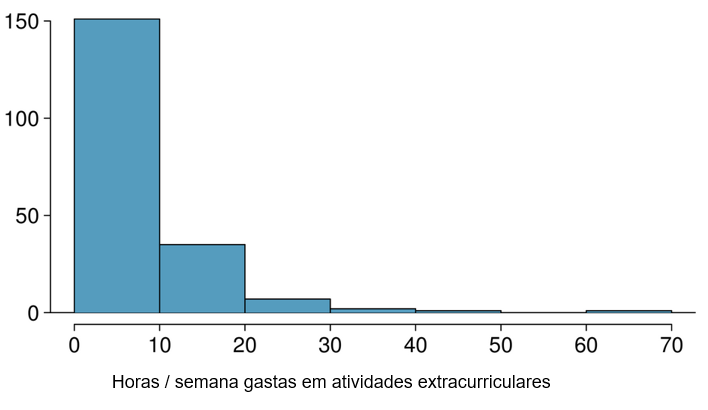
\includegraphics[width=0.75\textwidth]{1-6_numerical_data/extracurr_hrs_hist.png}
\end{center}
\justifying
\soln{\pause{Unimodal e assimétrica à direita. Outlier, às 60 horas/semana.}}

\end{frame}

%%%%%%%%%%%%%%%%%%%%%%%%%%%%%%%%%%%%

\begin{frame}
\frametitle{Formas comumente observadas de distribuições}

\begin{itemize}

\item modalidade \\
$\:$ \\
\pause

\begin{columns}[c]
\column{0.25\textwidth}
unimodal \\
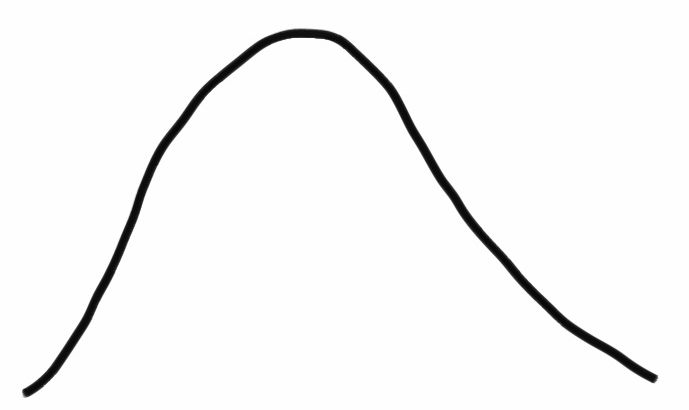
\includegraphics[width=\textwidth]{1-6_numerical_data/unimodal.png} 
\pause
\column{0.25\textwidth}
bimodal \\
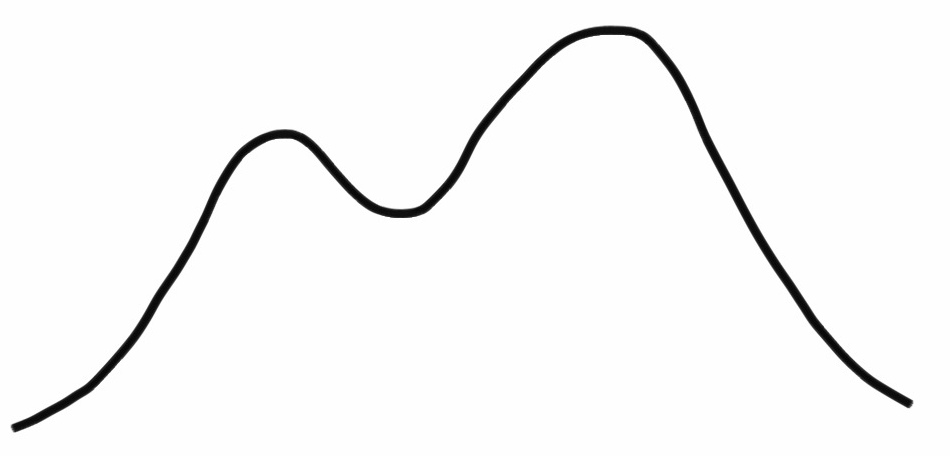
\includegraphics[width=\textwidth]{1-6_numerical_data/bimodal.png} 
\pause
\column{0.25\textwidth}
multimodal \\
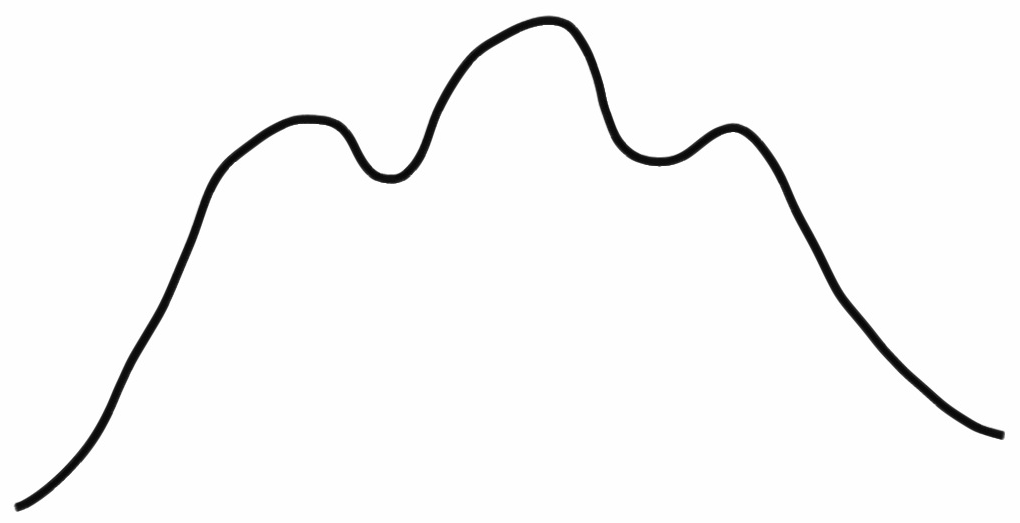
\includegraphics[width=\textwidth]{1-6_numerical_data/multimodal.png} 
\pause
\column{0.25\textwidth}
uniforme
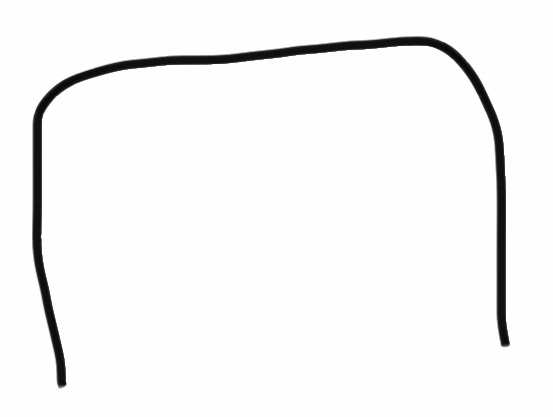
\includegraphics[width=\textwidth]{1-6_numerical_data/uniform.png} 
\end{columns}

\pause

$\:$ \\

\item assimétrica \\
$\:$ \\
\pause

\begin{columns}[c]
\column{0.25\textwidth}
à direita \\
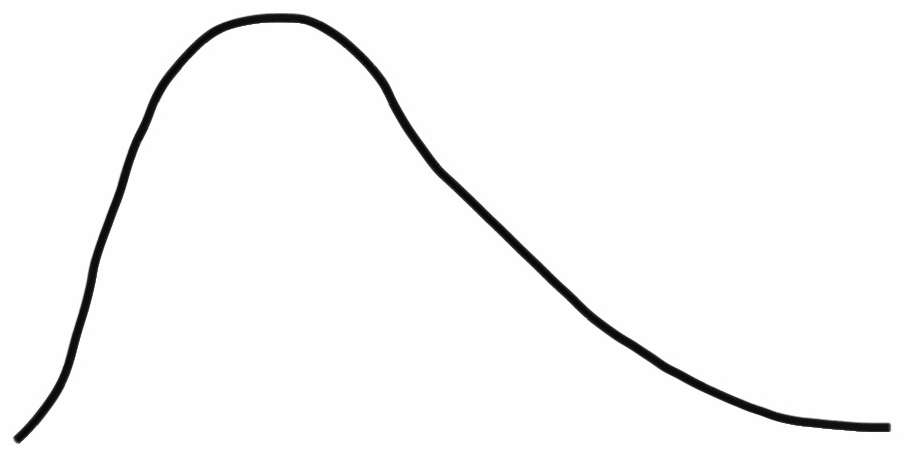
\includegraphics[width=\textwidth]{1-6_numerical_data/figures/shape_sketches/right_skew.png} 
\pause
\column{0.25\textwidth}
à esquerda \\
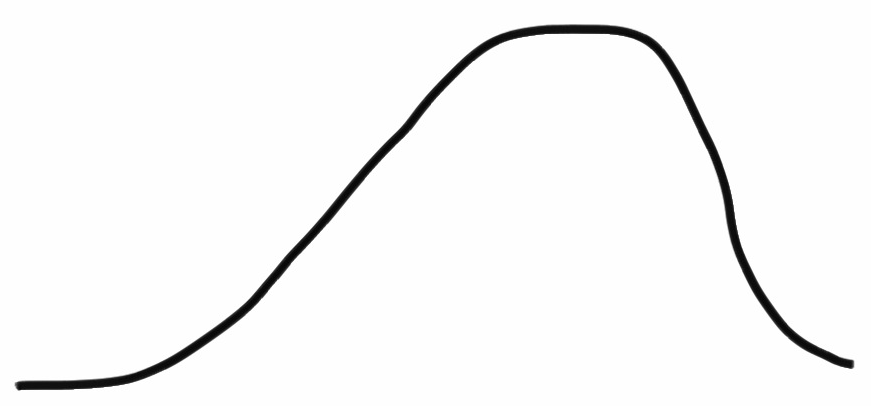
\includegraphics[width=\textwidth]{1-6_numerical_data/figures/shape_sketches/left_skew.png} 
\pause
\column{0.25\textwidth}
simétrico \\
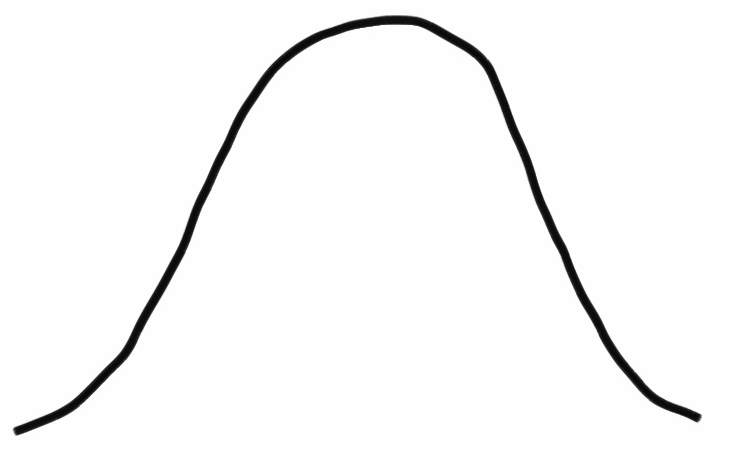
\includegraphics[width=\textwidth]{1-6_numerical_data/figures/shape_sketches/symmetric.png} 
\end{columns}

\end{itemize}

\end{frame}

%%%%%%%%%%%%%%%%%%%%%%%%%%%%%%%%%%%

\begin{frame}
\frametitle{Prática}

\pq{Quais dessas variáveis você espera que sejam uniformemente distribuídas?}

\begin{enumerate}[(a)]
\item pesos de habitantes de determinada cidade
\item salários de uma amostra aleatória de pessoas de Porto Alegre
\item Preços de casas
\solnMult{aniversários de colegas de turma (dia do mês)}
\end{enumerate}

\end{frame}

%%%%%%%%%%%%%%%%%%%%%%%%%%%%%%%%%%%

\begin{frame}
\frametitle{Atividade: formas de distribuições}

\app{Esboce as distribuições esperadas das seguintes variáveis:
\begin{itemize}
\item número de piercings
\item pontuações em um exame
\item Pontuações de QI
\end{itemize}
Invente uma maneira simples (1-2 sentenças) de ensinar alguém a determinar a distribuição esperada de qualquer variável.
}

\end{frame}

%%%%%%%%%%%%%%%%%%%%%%%%%%%%%%%%%%%

\begin{frame}
\frametitle{Você é típico? Qual seria o rosto médio de uma pessoa hoje?}

\begin{center}
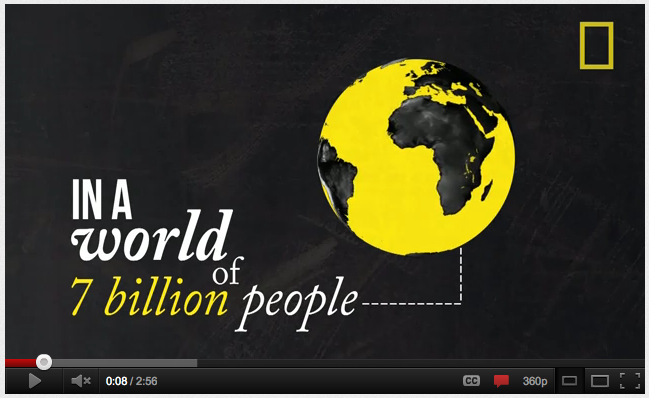
\includegraphics[width=0.75\textwidth]{1-6_numerical_data/figures/typical.png}
\end{center}

\begin{center}
\footnotesize{\webURL{http://www.youtube.com/watch?v=4B2xOvKFFz4}}
\end{center}


\end{frame}

%%%%%%%%%%%%%%%%%%%%%%%%%%%%%%%%%%%%

\subsection{Variância e desvio padrão}

%%%%%%%%%%%%%%%%%%%%%%%%%%%%%%%%%%%

\begin{frame}
\frametitle{Variância}
\justifying
\hl{Variância} é a soma dos desvios com relação à média ao quadrado.

\formula{
\[ s^2 = \frac{\sum_{i = 1}^n (x_i - \bar{x})^2}{n - 1} \]
}

\pause

\twocol{0.5}{0.5}
{
\begin{itemize}
\justifying
\item A média da amostra é $\bar{x} = 6,71$, e o tamanho da amostra é $n = 217$.
\justifying
\onslide<3->{\item A variação da quantidade de horas que estudantes dormem por noite pode ser calculada como:}
\end{itemize}
}
{
\onslide<2->{
\begin{center}
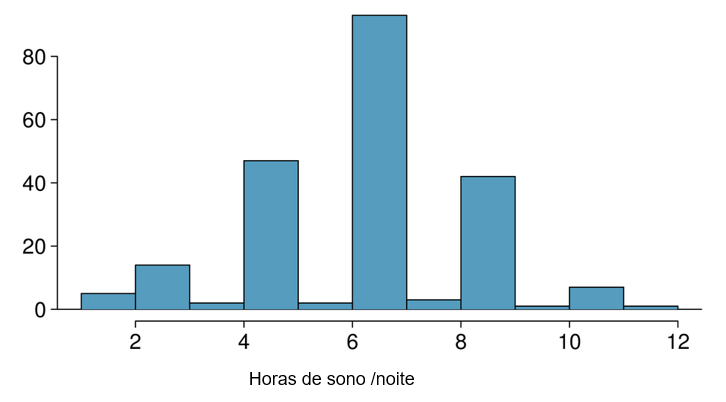
\includegraphics[width=\textwidth]{1-6_numerical_data/sleep_hist.png}
\end{center}
}
}
$\:$
\onslide<3->{
\[ s^2 = \frac{(5 - 6.71)^2 + (9 - 6.71)^2 + \cdots + (7 - 6.71)^2}{217 - 1} = 4.11~horas^2 \]
}



\end{frame}

%%%%%%%%%%%%%%%%%%%%%%%%%%%%%%%%%%%

\begin{frame}
\frametitle{Variância}
\justifying
\dq{Por que usamos o desvio ao quadrado no cálculo da variância?}

\soln{\pause
\begin{itemize}
\justifying
\item Para que as observações igualmente distantes da média sejam igualmente ponderadas, independentemente de essas distâncias serem positivas ou negativas.
\justifying
\item Para pesar desvios maiores mais fortemente.
\justifying
\item Porque as soma dos desvios em relação à média é zero


\end{itemize}
}

\end{frame}

%%%%%%%%%%%%%%%%%%%%%%%%%%%%%%%%%%

\begin{frame}
\frametitle{Desvio padrão}

\justifying
O \hl{desvio padrão} é a raiz quadrada da variância e possui a mesma unidade de medida dos dados observados.
$$
 s = \sqrt{s^2} 
$$
\pause
\twocol{0.5}{0.5}
{
\begin{itemize}
\justifying
\item O desvio padrão da quantidade de horas que estudantes dormem por noite é calculado como:
$$
 s = \sqrt{4.11} = 2.03~horas
$$
\justifying
\end{itemize}
}
{
\onslide<2->{
\begin{center}
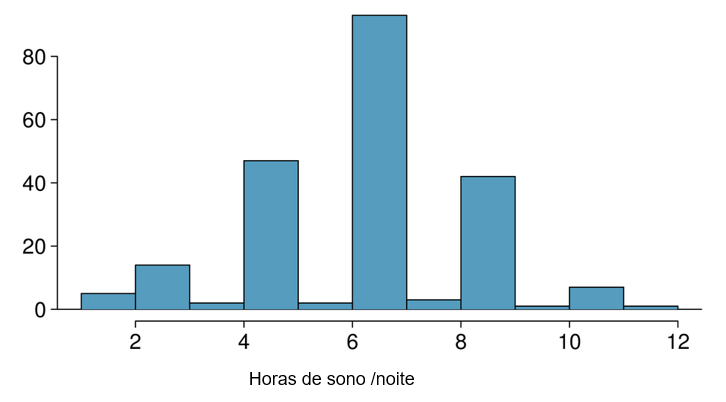
\includegraphics[width=\textwidth]{1-6_numerical_data/sleep_hist.png}
\end{center}
}
}

\end{frame}
%%%%%%%%%%%%%%%%%%%%%%%%%%%%%%%%%%

\begin{frame}
\frametitle{Desvio padrão}

\begin{itemize}
\justifying
$$
 s = \sqrt{4.11} = 2.03~horas
$$
\justifying
\item Observe que todas as observações estão dentro do intervalo de até 3 desvios padrões da média.
\end{itemize}
\begin{eqnarray*}
    (\overline{x}- 3s  &;& \overline{x}+ 3s)\\
     (6,71 -3\times2,03 &;& 6,71 +3\times2,03)
\end{eqnarray*}

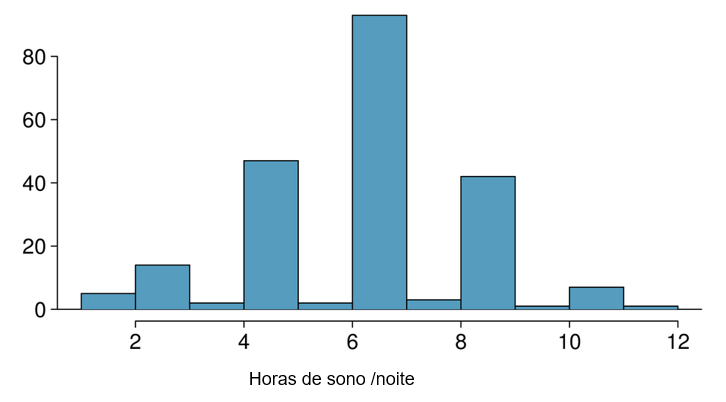
\includegraphics[width=6cm]{1-6_numerical_data/sleep_hist.png}

\end{frame}

%%%%%%%%%%%%%%%%%%%%%%%%%%%%%%%%%%%%

\subsection{Boxplot, quartis e a mediana}

%%%%%%%%%%%%%%%%%%%%%%%%%%%%%%%%%%%%

\begin{frame}
\frametitle{mediana}

\begin{itemize}
\justifying
\item A \hl{mediana} é o valor que divide  os dados ordenados pela metade.

\[ 0,1,\orange{2},3,4 \]
\justifying
\item Se houver um número par de observações, a mediana é a média dos dois valores do meio.

\[ 0,1,\underline{2,3},4,5 \rightarrow \frac{2 + 3}{2} = \orange{2.5} \]
\justifying
\item Como a mediana é o ponto médio dos dados, 50\% dos valores estão abaixo dela. Por isso, é também o \hl{percentil $50$}.

\end{itemize}

\end{frame}

%%%%%%%%%%%%%%%%%%%%%%%%%%%%%%%%%%%%

\begin{frame}[fragile]
\frametitle{Q1, Q3, and IQR}

\begin{itemize}
\justifying
\item O $25^{0}$ percentil também é chamado  primeiro quartil, \hl{Q1}.
\justifying
\item O $50^{0}$ percentil também é chamado de mediana.
\justifying
\item O $75^{0}$ percentil também é chamado terceiro quartil, \hl{Q3}.
\justifying
\item Entre Q1 e Q3 está 50\% dos dados. O intervalo desses dados é chamado de \hl{intervalo interquartílico} ou \hl{IQR}.

$$
IQR = Q3 - Q1 
$$

\end{itemize}

\end{frame}

%%%%%%%%%%%%%%%%%%%%%%%%%%%%%%%%%%%%

\begin{frame}
\frametitle{Boxplot}
\justifying
A caixa em um \hl{boxplot} representa 50\% dos dados e a linha que corta a caixa representa a \hl{mediana}.

\begin{center}
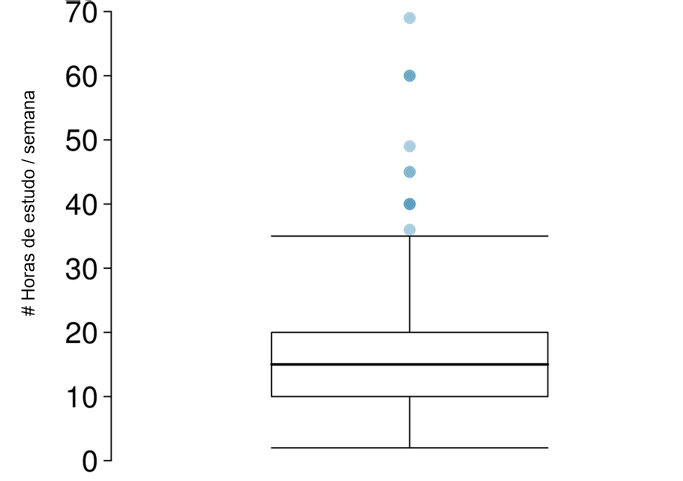
\includegraphics[width=0.7\textwidth]{1-6_numerical_data/study_hours_box.png}
\end{center}

\end{frame}

%%%%%%%%%%%%%%%%%%%%%%%%%%%%%%%%%%%%

\begin{frame}
\frametitle{Explicando um boxplot}

\begin{center}
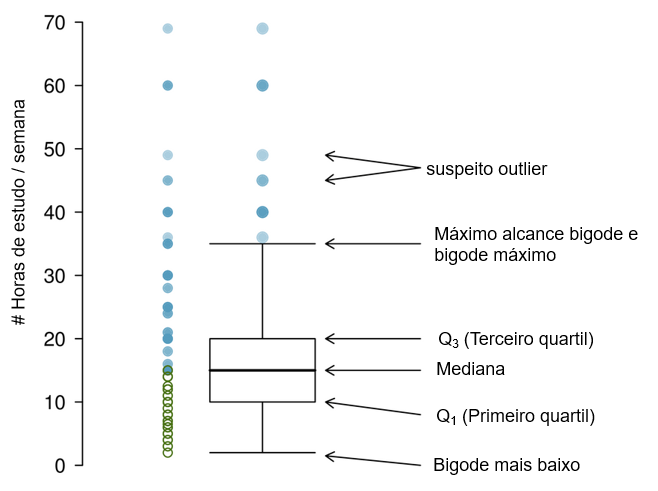
\includegraphics[width=0.95\textwidth]{1-6_numerical_data/study_hours_box_layout.png}
\end{center}

\end{frame}

%%%%%%%%%%%%%%%%%%%%%%%%%%%%%%%%%%%%

\begin{frame}[fragile]
\frametitle{Bigodes e outliers}

\begin{itemize}
\justifying
\item \hl{Bigodes} de um gráfico de caixa podem se estender até $1.5 \times IQR$ longe dos quartis.\\
\formula{
\vspace{-0.5cm}
\begin{align*} 
\text{alcance~máximo~bigode~superior} &= Q3 + 1.5 \times IQR \\
\text{alcance~máximo~bigode~inferior~} &= Q1 - 1.5 \times IQR
\end{align*}
}
\pause
\vspace{-0.5cm}
{\small
\begin{align*}
\text{IQR}&: 20 - 10 = 10 \\
\text{alcance~máximo~bigode~superior}&= 20 + 1.5 \times 10 = 35 \\
\text{alcance~máximo~bigode~inferior}&= 10 - 1.5 \times 10 = -5
\end{align*}
}

\pause
\vspace{-0.25cm}
\justifying
\item Um potencial \hl{outlier} é definido como uma observação além do alcance máximo dos bigodes. É uma observação que parece extrema em relação ao resto dos dados.

\end{itemize}

\end{frame}

%%%%%%%%%%%%%%%%%%%%%%%%%%%%%%%%%%%%

\begin{frame}
\frametitle{Outliers (cont.)}
\justifying
\dq{Por que é importante procurar outliers?}

\soln{
\onslide<2->{
\begin{itemize}
\justifying
\item Identifica distorções na distribuição.
\justifying
\item Identifica erros ao construir o banco de dados e na coleta de dados.
\justifying
\item Fornece informações sobre características interessantes nos dados.
\end{itemize}
}
}

\end{frame}

%%%%%%%%%%%%%%%%%%%%%%%%%%%%%%%%%%%%

\subsection{Estatísticas robustas}

%%%%%%%%%%%%%%%%%%%%%%%%%%%%%%%%%%%%

\begin{frame}
\frametitle{Observações extremas}
\justifying
\dq{Como estatísticas como média, mediana, desvio padrão e IQR da renda familiar seriam afetadas se o maior valor fosse substituído por \$ 10 milhões? E se o menor valor fosse substituído por \$ 10 milhões?}

\begin{center}
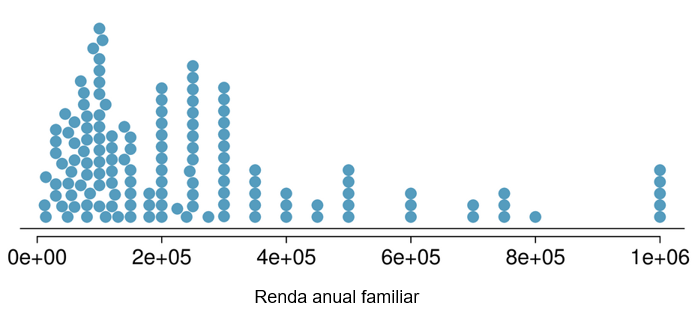
\includegraphics[width=\textwidth]{1-6_numerical_data/house_income_dot_stacked.png}
\end{center}

\end{frame}

%%%%%%%%%%%%%%%%%%%%%%%%%%%%%%%%%%%%

\begin{frame}
\frametitle{Estatísticas robustas}

\begin{center}
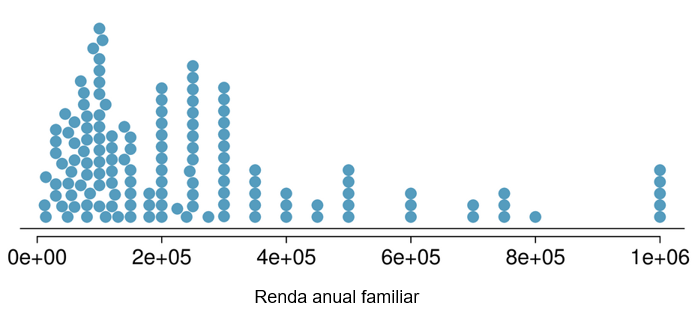
\includegraphics[width=\textwidth]{1-6_numerical_data/house_income_dot_stacked.png}
\end{center}
\end{frame}
%%%%%%%%%%%%%%%%%%%%%%%%%%%%%%%%%%%%

\begin{frame}
\frametitle{Estatísticas robustas}

\begin{center}
\scalebox{0.9}{
\begin{tabular}{l c cc c cc}
  \hline

& \hspace{0mm} & \multicolumn{2}{c}{\bf robusta} & \hspace{2mm} & \multicolumn{2}{c}{\bf não robusta} \\
cenário && mediana & IQR && $\bar{x}$ & $s$ \\ 
  \hline
dados originais && 190K & 200K && 245K & 226K \\ 
substituir o maior valor por  && 190K & 200K && 309K & 853K \\
\$10 milhões & & & & \\
substituir o menor valor 
 && 200K & 200K && 316K & 854K \\
 por \$10 milhões & & & & \\
   \hline
\end{tabular}
}
\end{center}


\end{frame}

%%%%%%%%%%%%%%%%%%%%%%%%%%%%%%%%%%%%

\begin{frame}
\frametitle{Estatísticas robustas}
\justifying
A mediana e o IQR são mais robustas à assimetria e aos desvios do que a média e o desvio padrão. Assim sendo,

\begin{itemize}
\justifying
\item Para distribuições muito assimétricas, é mais útil usar mediana e IQR para descrever o centro e a variabilidade.
\justifying
\item Para distribuições simétricas, é mais útil usar a média e o desvio-padrão para descrever o centro e a variabilidade.
\end{itemize}

$\:$ \\

\pause
\justifying
\dq{Se você quiser estimar a renda familiar típica de um aluno, você estaria mais interessado na renda média ou mediana?}

\soln{\pause{Mediana}}

\end{frame}

%%%%%%%%%%%%%%%%%%%%%%%%%%%%%%%%%%%%

\begin{frame}
\frametitle{Média vs. mediana}

\begin{itemize}
\justifying
\item Se a distribuição é simétrica, o centro é geralmente definido como a média: média $\approx$ mediana

\begin{center}
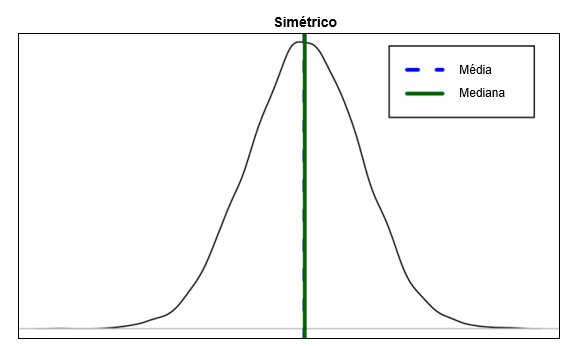
\includegraphics[width=0.6\textwidth]{1-6_numerical_data/sym.png}
\end{center}

\end{itemize}

\end{frame}
%%%%%%%%%%%%%%%%%%%%%%%%%%%%%%%%%%%%

\begin{frame}
\frametitle{Média vs. mediana}

\begin{itemize}
\justifying
\item Se a distribuição é assimétrica ou tem outliers, o centro é geralmente definido como a mediana
\begin{itemize}
\item Assimétrico à direita: média $>$ mediana
\item Assimétrico à esquerda: média $<$ mediana \\
\end{itemize}

\end{itemize}

\begin{center}
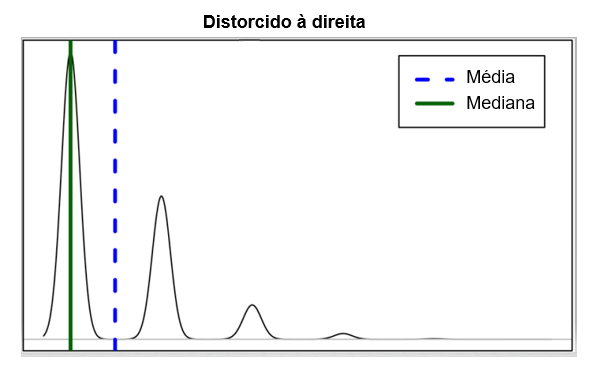
\includegraphics[width=0.5\textwidth]{1-6_numerical_data/rs.png}
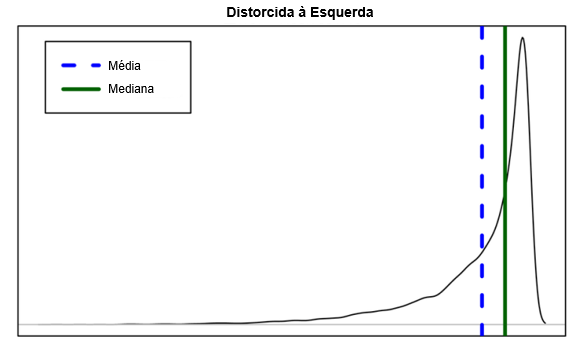
\includegraphics[width=0.5\textwidth]{1-6_numerical_data/ls.png}\\
\end{center}

\end{frame}

%%%%%%%%%%%%%%%%%%%%%%%%%%%%%%%%%%%%%

\begin{frame}
\frametitle{Prática}
\justifying
\pq{{\small O que é mais provável que seja verdade sobre a distribuição da porcentagem de tempo gasto com anotações em sala de aula em comparação com o Facebook, o Twitter etc.?}}

\vspace{-0.5cm}

\begin{columns}
\column{0.7\textwidth}
\begin{center}
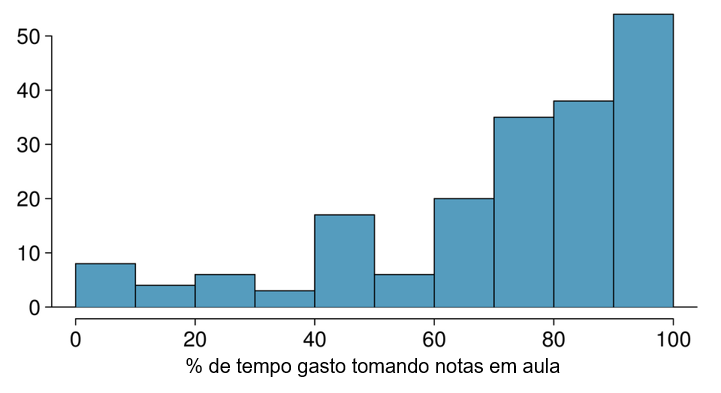
\includegraphics[width=0.9\textwidth]{1-6_numerical_data/notes_perc_hist.png}
\end{center}
\column{0.3\textwidth}
$\:$ \\
$\:$ \\
\soln{\only<2>{\orange{mediana: 80\% \\ média: 76\%}}}
\end{columns}

{\small
\begin{multicols}{2}
\begin{enumerate}[(a)]
\item média $>$ mediana
\solnMult{média $<$ mediana}
\item média $\approx$ mediana
\item impossível dizer
\end{enumerate}
\end{multicols}
}

\end{frame}

%%%%%%%%%%%%%%%%%%%%%%%%%%%%%%%%%%%%%

\subsection{Transformando dados}

%%%%%%%%%%%%%%%%%%%%%%%%%%%%%%%%%%%%

\begin{frame}
\frametitle{Dados extremamente assimétricos}
\justifying
Quando os dados são extremamente assimétricos, transformá-los pode facilitar a modelagem. Uma transformação comum é a \hl{transformação log}.

$\:$ \\
\pause
\justifying
O histograma à esquerda mostra a distribuição do número de jogos de basquete assistidos pelos alunos. O histograma à direita mostra a distribuição do \hl{log} do número de jogos assistidos.

\begin{center}
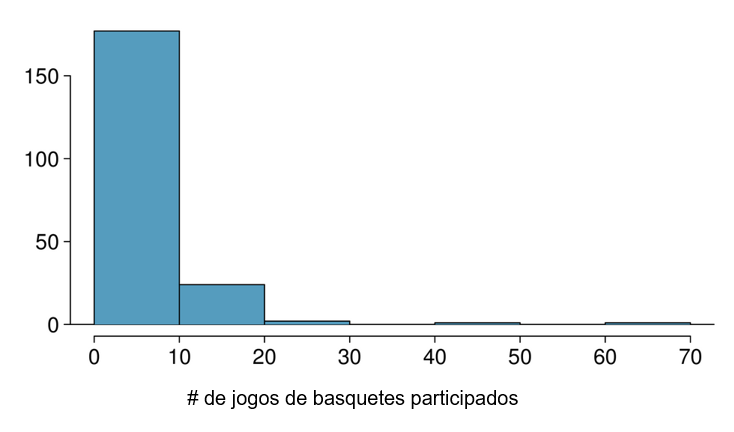
\includegraphics[width=0.5\textwidth]{1-6_numerical_data/basket_games_hist.png}
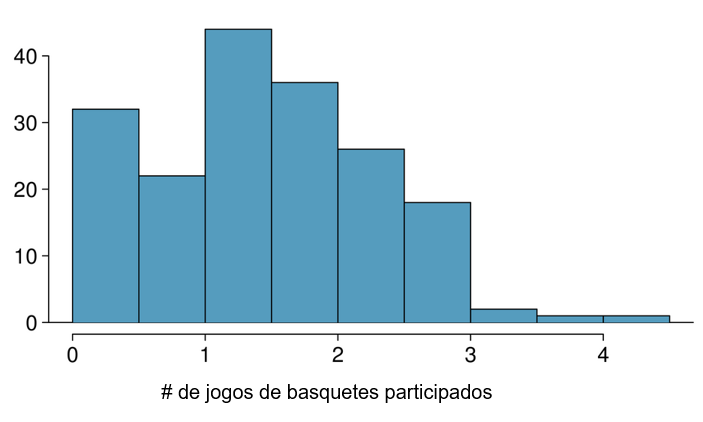
\includegraphics[width=0.5\textwidth]{1-6_numerical_data/basket_games_hist_log.png}
\end{center}

\end{frame}

%%%%%%%%%%%%%%%%%%%%%%%%%%%%%%%%%%%%

\begin{frame}
\frametitle{Prós e contras de transformações}

\begin{itemize}
\justifying
\item Os dados assimétricos são mais fáceis de modelar quando são transformados, porque os outliers tendem a se tornar bem menos proeminentes após uma transformação apropriada. \\
$\:$ \\
\renewcommand{\arraystretch}{1.5}
\begin{tabular}{l r r r r }
\# de jogos		&  70 	& 50 		& 25 		 		& $\cdots$ \\
log(\# de jogos)	& 4.25	& 3.91 	& 3.22 	 	& $\cdots$
\end{tabular}

$\:$ \\
\justifying
\item No entanto, os resultados de uma análise podem ser difíceis de interpretar porque o \hl{log} de uma variável medida é geralmente sem sentido.

\end{itemize}

\pause
\justifying
\small{
\dq{Quais outras variáveis você esperaria que fossem extremamente assimétricas?}

\soln{\pause{Salário, preços de imóveis, etc.}}
}
\end{frame}

%%%%%%%%%%%%%%%%%%%%%%%%%%%%%%%%%%%%

\subsection{Mapeando dados}

%%%%%%%%%%%%%%%%%%%%%%%%%%%%%%%%%%%%

\begin{frame}
\frametitle{Mapas de intensidade}
\justifying
\dq{Quais padrões são aparentes na mudança de população entre 2000 e 2010?}

\begin{center}
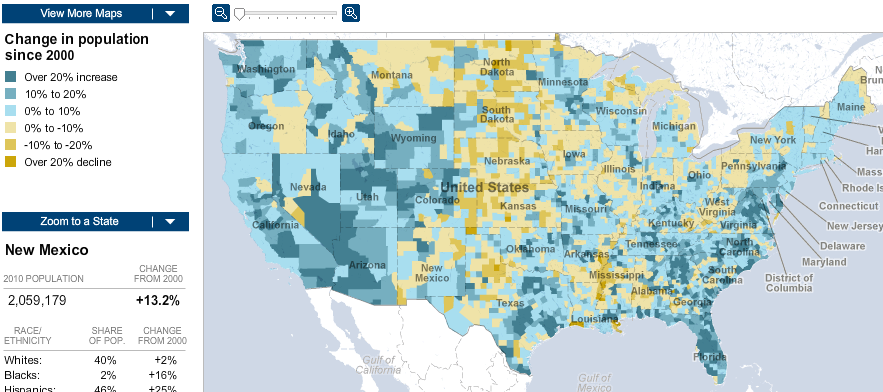
\includegraphics[width=0.95\textwidth]{1-6_numerical_data/change_in_pop_intensity.png}
\end{center}

\ct{\webURL{http://projects.nytimes.com/census/2010/map}}

\end{frame}


%%%%%%%%%%%%%%%%%%%%%%%%%%%%%%%%%%%%


